\chapter{Popis metody měření}
\label{sec:measurement}
Zjednodušená schéma vstupu / výstupu ATmega je zobrazeno na obrázku~\ref{fig:port}.
Přepínač PUD vypne napájení pro všechny ,,Pull Up'' odpory ATmega.
Pomocí přepínače DD lze výstup vypnout, vstup pracuje bud jako výstup, tak i jako vstup.
Ve vstupním režimu je výstupní hodnota (PORT) použita k přepnutí,,Pull Up'' odporu vstupu.
Ty dva přepínače PORT a DD nelze přepínat současně, ale pouze jeden po druhém.
Protože přepnutí ,,Pull Up'' odporu může rušit měření, dávám přednost úplnému
odpojení všech  ,,Pull Up'' odporů pomocí spínače PUD.
Samozřejmě, že jsou přepínače elektronické a odpory \(19\Omega\) a \(22\Omega\) jsou jen přibližné hodnoty.

\begin{figure}[H]
\centering
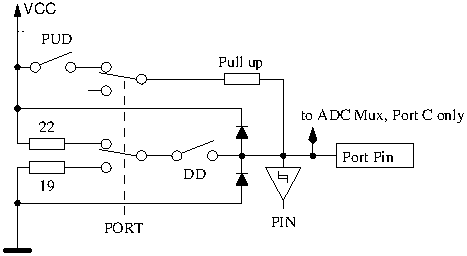
\includegraphics[width=.8\textwidth]{../FIG/port.pdf}
\caption{Zjednodušené schéma každého pinu ATmega portu}
\label{fig:port}
\end{figure}

Každý ze tří zkušebních pinů vašeho testeru se skládá ze tří pinů ATmega,
který je znázorněn na zjednodušeném schéma zkušebního čepu TP2 (prostřední ze tří pinů) na obrázku~\ref{fig:terminal}.

\begin{figure}[H]
\centering
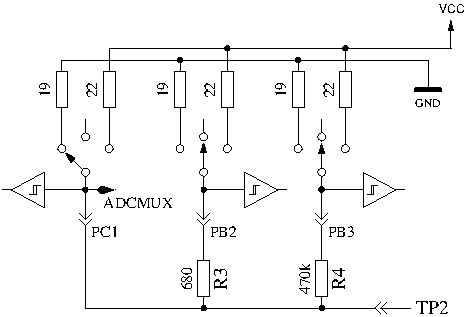
\includegraphics[width=.8\textwidth]{../FIG/terminal.pdf}
\caption{Zjednodušené schéma zapojení zkušebního pinu TP2}
\label{fig:terminal}
\end{figure}

Každý zkušební pin (měřící port) lze použít jako digitální nebo analogový vstup.
Tato schopnost měření je nezávislá na použití portu jako výstupu.
Každý zkušební pin může být použit jako výstup a připojen v tomto stavu k GND (\(0V\)) nebo VCC (\(5V\)),
nebo může být připojen buď k GND nebo VCC pomocí odporů (\(680\Omega\) nebo \(470k\Omega\)).
Tabulka \ref{tab:case} zobrazuje všechny možnosti měření.
Všimněte si, že pozitivní stav je dosažen připojením přímo k VCC (Port C) nebo
připojením k rezistoru \(680\Omega\) s VCC (Port B).
Stejná možnost má negativní stav zkušebního kolíku na straně GND.
Stav testu znamená, že pin může být otevřený (vstup) připojen pomocí odporu \(470k\Omega\) s VCC nebo GND,
nebo pin může být připojen k VCC nebo GND přes \(680\Omega\)-odpor.

\begin{table}[H]
  \begin{center}
    \begin{tabular}{| l | c | c | c |}
    \hline
      & Stav Pin 1 & Stav Pin 2 & Stav Pin 3 \\
    \hline
   1. & positivní    &  negativní   &  test \\
   2. & positivní    &  test      & negativní \\
   3. & test       &  negativní   & positivní \\
   4. & test       &  positivní   & negativní \\
   5. & negativní    &  test      & positivní \\
   6. & negativní    &  positivní   &  test  \\
    \hline
    \end{tabular}
  \end{center}
  \caption{všechny možnosti měření}
  \label{tab:case} 
\end{table}

Jakmile je nakonfigurováno měření kondenzátoru testerem,  pokusí se přístroj nejprve
k vybíjení kondenzátorů na všech připojovacích kolících.
Pokud to nefunguje, to znamená zbytkové napětí je příliš vysoké, bude vybíjení
po cca 12 sekundách přerušeno se zprávou ,,Cell!''.

To se může stát i v případě když není žádný kondenzátor připojen.

Příčinou může v tomto případě být, že je mezní napětí výboje pro tento
ATmega příliš nízké.\\ Pomocí makefile volby CAP\_EMPTY\_LEVEL, můžete ale zvolit vyšší zbytkové napětí.
